%\dunja{extend the section title to make a clear distinction form Section5: ``''Implementation Details"}
StreamStory is implemented as a client-server application with a web-based user interface. %implemented %using the state-of-the-art technologies such as HTML5, CSS3 and JavaScript. 
The layout is handled by Twitter Bootstrap 3, %, providing responsiveness and scalability to most modern device sizes,
while the controller is implemented using jQuery, providing cross-browser support. We use Cytoscape.js for visualization of graphs and trees, including the main visualization panel, and D3.js for visualization of histograms. %The controller relies on technologies like Ajax and WebSockets for transparent interactive updates.
%
The backend uses a hybrid implementation with its core functionality written in C++, as part of the QMiner data analytics platform \cite{qminer}. This functionality is exposed as a Node.js addon running in Googles V8 JavaScript environment. 
%Node.js thus acts as glue and exposes the core functionality through RESTful web services using the Express framework, also acting as the session manager. User credentials and other information are stored in a MySQL database.

%Having the core functionality implemented in C++ provides performance benefits, especially
%when dealing with larger datasets. When using StreamStory, 
We found the most time consuming step
is model initialization. Indeed, after this initial step, everything is fully interactive.
The initialization includes partitioning the dataset, aggregating states, modeling transitions,
computation of state statistics, initialization of state assistance services and laying out the generated
hierarchical graph onto a plane. Our experiments show that within the initialization step, the most time-consuming of these tasks are the state assistance services. A decision tree and a logistic regression
model must be computed for each state in the hierarchical structure. These state initialization tasks
are independent and can potentially be parallelized.

To measure the performance of the initialization procedure, we constructed several models on two datasets of sizes $155MB$ ($\approx 285k$ samples) and $500MB$ ($\approx 3M$ samples) respectively. A set of five attributes
was randomly chosen for each dataset and was used in all the experiments. We then constructed models with 18, 38 and 78 states respectively and measured the initialization times, which we show in Figure \ref{fig:performance}.
\begin{figure}[h!]
	\centering
	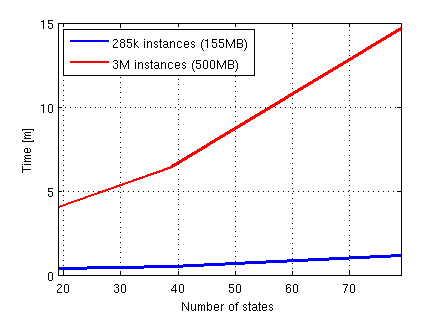
\includegraphics[width=0.7\columnwidth]{time-measurements}
	\caption{A chart showing the dependence of model construction time to the dataset size and the number of states used in the model. \lstopar{From the chart we can see a clear dependence between the construction time and the number of states for \textcolor{red}{large} datasets}.}
	\label{fig:performance}
\end{figure}
We can see that although the construction time increases with the number of states, the initialization
procedure is quite fast for the smaller data set with only the larger model with 78 states taking over 
a minute to complete. When using the larger dataset, the dependence between the number of states and the construction time becomes clearer with the model with $18$ states taking less than $5$ minutes to complete while the larger model taking just under $15$ minutes.

% \lstopar{
% \begin{itemize}
% 	\item the larger dataset was constructed in acceptable time
% 	\item theoretically the dependence should be $O(n^2)$
% \end{itemize}
% }

\iffalse
\begin{tabular}{ c | c c c c c}
	\label{tab:time-tests}
	 & 10 & 20 & 40 & reading CSV & file size \\
	\hline
	3229541 & 11min & 13min 32s & 21min 50s & 6:58,7:05,7:10 & 500MB \\
	285168 & 1:31 & 1:36 & 2:17 & 1:09,1:06,1:08 & 155MB
\end{tabular}
\fi